%----------------------------------------------------------------------------------------------------------------------------------------------------------%
\chapter{Experimental design}
%----------------------------------------------------------------------------------------------------------------------------------------------------------%
\epigraph{It is common sense to take a method and try it; if it fails, admit it frankly and try another. But above all, try something.}{\textit{Anthony Burgess}}
%----------------------------------------------------------------------------------------------------------------------------------------------------------%
\paragraph{}This Extended Essay has the objective of studying bibliographically the effects of \emph{Staphylococcus aureus} on the human body, as well as the ways humanity has developed to defeat it. Experimentally, it has one main objective, and several secondary ones: answering the research questions posed in the most reliable way I can achieve. Secondarily, I want to improve my lab etiquette and fluidity, protocol-making, how I follow protocols in the lab and how I deal with problems that may arise from them, my staining and microscope use,  and how I work with limited resources.\newline 
The research question I will follow is 
\begin{center}"\emph{What is the prevalence of \emph{Staphylococcus aureus} in our school}?"\end{center}
To which my hypothesis is:
\begin{center}\emph{``About 30\%``}\end{center} 
This hypothesis stems from results I found in my bibliographical research. I would also like to know the answer to the question
\begin{center}"\emph{Is the prevalence of \emph{Staphylococcus aureus} affected by gender or age?}"\end{center}
to which my hypothesis is 
\begin{center}\emph{``No``}\end{center}
The variable I will study is the presence or not of the bacterium in question on different subjects, and compare it against their characteristics (such as approximate age and gender). I'll keep constant the culture medium, as well as the culture temperature and humidity.
%----------------------------------------------------------------------------------------------------------------------------------------------------------%
\section{Variables studied}
\paragraph{}This study studied one dependent variable: the prevalence of \emph{Staphylococcus aureus}, comparing it against two different independent variables: the gender of the subject and the age group of the subject. This will allow me to check for a correlation between these tw
%----------------------------------------------------------------------------------------------------------------------------------------------------------%
\section{Bill of materials}
\paragraph{}The materials used, as well as the quantities used, can be found in the following table. On the left, laboratory equipment and, on the right, reagents, staining agents, and consumables used:
\begin{center}\begin{figure}[H]\centering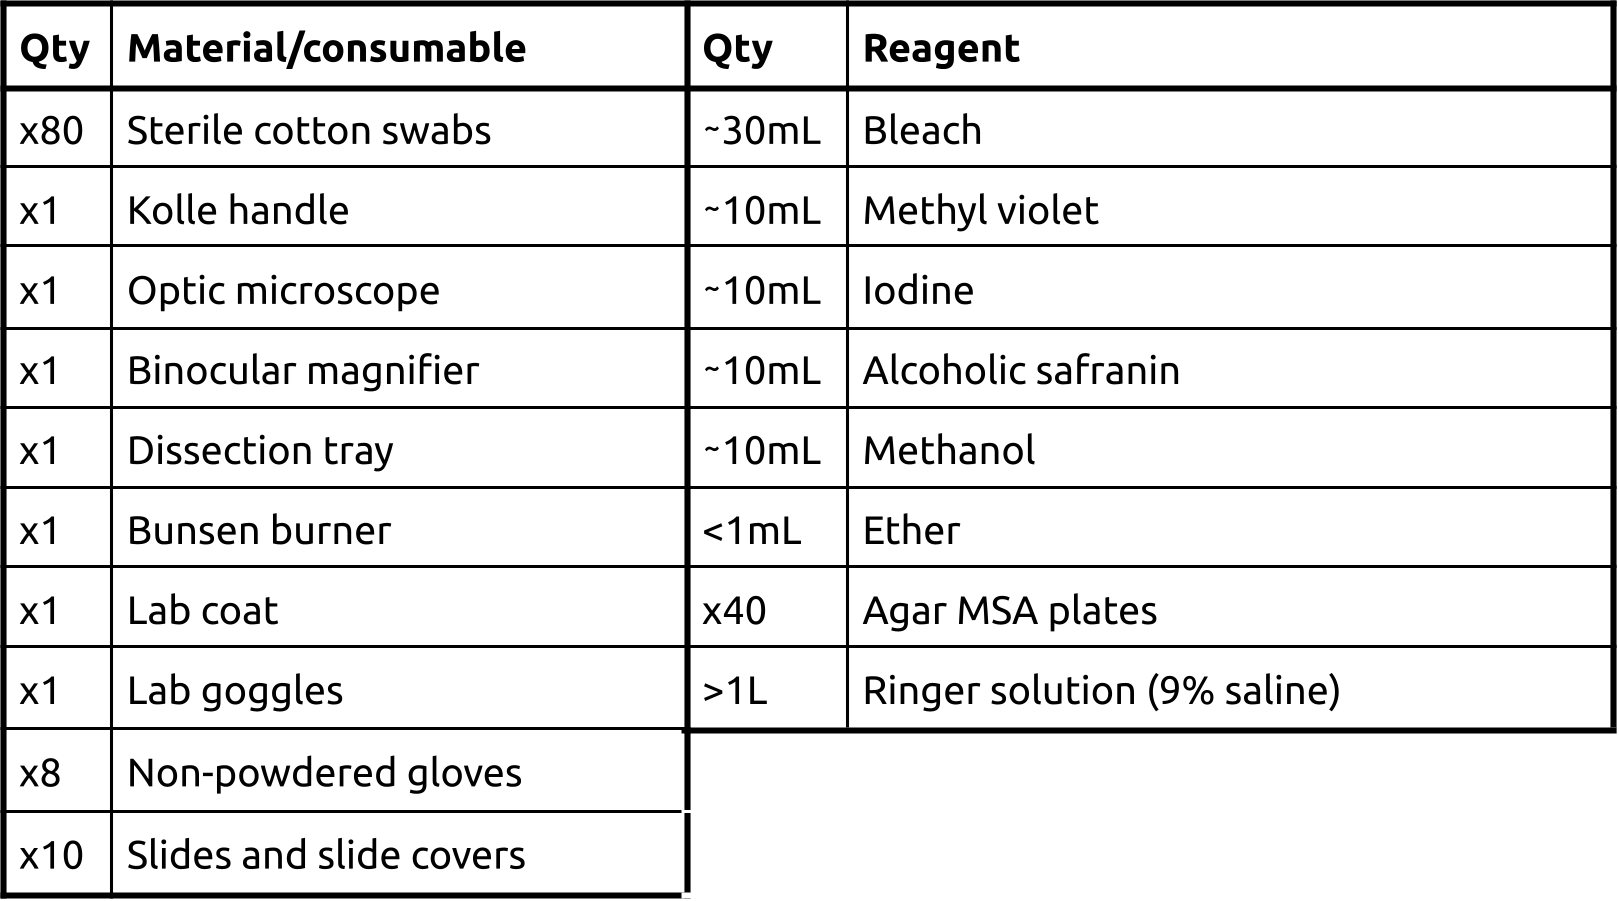
\includegraphics[width=0.90\textwidth]{BOM-1.png}\end{figure}\end{center}
%----------------------------------------------------------------------------------------------------------------------------------------------------------%
\section{Biosecurity and risk mitigation}
\paragraph{}Staph is considered a Biosecurity Level 2 bacterium\cite{cheungPathogenicityVirulenceStaphylococcus2021}. This means that it is associated with a human disease that can pose a moderate human health hazard. In a laboratory where such individua are handled, normal lab etiquette should be followed, as well as avoiding splashes or aerosols, adhering biohazard warning signs present on all material used, and proper surfaces and material disinfection via the use of autoclave.\newline
The risks associated with this bacterium were assessed following the 2020 Biosafety Manual published by the WHO, and proper security measures were followed at all times when handling biohazardous material. No incidents occurred during the research\cite{worldhealthorganizationLaboratoryBiosafetyManual2020}.\newpage